In this chapter in \cref{exp:model_tests} we evaluate the proposed heuristic against the MILP model (\ref{sec:milp}) and in \cref{exp:literature_tests} against other heuristic from the literature. We then show the effectivness of our approach for our case study in \cref{exp:usecase_results}.
All the tests were run on a desktop computer with an AMD Ryzen-7 5800x processor with 8 cores at 3.8 GHz and 32GB of DDR4 system RAM with Windows 10. The algorithm was implemented in Java 11 and the model was run using the python APIs from CPLEX Optimization Studio 22.1.0.
In every test CPLEX was used with a maximum runtime of 1 hour.
Each evaluation against the heuristic lists both operational modes described in \cref{sec:placement_modes} and are listed as "Order By Hash" and "Single Placement".

%TODO: Talk about time normalization?
\section{Model validation}
We compared our heuristic to the proposed MILP model of \cref{sec:milp} with a single bin and with no limit on the height of the bin (also referred to the 3D strip packing problem).
The heuristic was configured to run without vertex support, using only area support rules for its feasibility checks and $k$ was set to $200$.
The configured parameters for the test were $\alpha_s = 0.7$, $\beta_s = 5$, and the discretization unit for the model was $\delta = 10$. 
Tests were run on the first instance of the class 1 problems of the literature tests described in \cref{def:class1_instances}.
The test was run with an iterative approach by selecting only a limited ammout of items from the selected instance starting from 1 item and increasing the number of items to pack by one at each iteration.
Starting from instance with 6 boxes to pack, the solution from the previous instance of the problem was used to mip start the new one to allow for lower execution times.
Table \ref{exp:model} shows the obtained $z_{\text{max}}$ value of the heuristic and the MILP solution, the runtime in seconds and the number of items.
Since the underlying problem is NP-Hard it is shown that starting from instances of size bigger than 8 items, the MILP model becomes too slow for practical use while our heuristic mantains a negligible execution time.
Due to discretization errors, some of the model instances gave solutions that didn't have the expected ammount of support and are marked with an asterix.
All the instaces divided by number of items are available at \url{https://github.com/artumino/BinPackingThesis/tree/main/tests/model/instances}.
The solution to instance number 5 and instance number 7 is also shown in \cref{fig:model_tests}.
\label{exp:model_tests}
\begin{table}[htbp]
    \centering
    \caption{Comparison with MILP model on limited set of boxes}
    \begin{tabular}{|c|c|c|c|c|c|c|c|}
    \hline
    & \multicolumn{ 3}{c|}{\textbf{MILP Model}} & \multicolumn{ 2}{c|}{\textbf{PM}} & \multicolumn{ 2}{c|}{\textbf{PS}} \\ \hline
    \textbf{$n$} & \textbf{Max Z} & \textbf{TT(s)} & \textbf{Gap($\%$)} & \textbf{Max Z} & \textbf{TT(s)} & \textbf{Max Z} & \textbf{TT(s)} \\ \hline
    1  & 85   & 0.01     & 0.00 & 85  & 0.00 & 85  & 0.00 \\ 
    2  & 85   & 0.07     & 0.00 & 85  & 0.00 & 85  & 0.00 \\ 
    3  & 85   & 0.13     & 0.00 & 85  & 0.00 & 85  & 0.00 \\ 
    4  & 85   & 0.20     & 0.00 & 85  & 0.01 & 85  & 0.01 \\ 
    5  & 85   & 2.02     & 0.00 & 85  & 0.02 & 85  & 0.02 \\ 
    6  & 158  & 90.58    & 0.00 & 158 & 0.06 & 158 & 0.05 \\ 
    7  & 158  & 1,369.24 & 0.00 & 158 & 0.07 & 158 & 0.08 \\ 
    8  & 161* & 3,600.00 & 1.86 & 160 & 0.10 & 160 & 0.08 \\ \hline
    9  & -    & -        & -    & 169 & 0.09 & 161 & 0.10 \\ 
    10 & -    & -        & -    & 218 & 0.12 & 218 & 0.13 \\ 
    11 & -    & -        & -    & 240 & 0.12 & 240 & 0.12 \\ 
    12 & -    & -        & -    & 310 & 0.13 & 316 & 0.16 \\ 
    13 & -    & -        & -    & 310 & 0.15 & 333 & 0.18 \\ 
    14 & -    & -        & -    & 310 & 0.20 & 333 & 0.22 \\ 
    15 & -    & -        & -    & 406 & 0.21 & 397 & 0.27 \\ 
    16 & -    & -        & -    & 435 & 0.23 & 452 & 0.36 \\ 
    17 & -    & -        & -    & 429 & 0.27 & 515 & 0.41 \\ 
    18 & -    & -        & -    & 432 & 0.32 & 522 & 0.47 \\ 
    19 & -    & -        & -    & 458 & 0.35 & 522 & 0.55 \\ 
    20 & -    & -        & -    & 539 & 0.37 & 564 & 0.62 \\ \hline
    \end{tabular}
    \label{exp:model}
    \caption*{* Some boxes had lower support than expected due to discretization errors.}
    \end{table}

\begin{table}[htbp]
    \centering
    \caption{Comparison with MILP model on limited set of boxes}
    \begin{tabular}{|c|c|c|c|c|c|c|c|}
    \hline
    & \multicolumn{ 3}{c|}{\textbf{MILP Model}} & \multicolumn{ 2}{c|}{\textbf{PM}} & \multicolumn{ 2}{c|}{\textbf{PS}} \\ \hline
    \textbf{$n$} & \textbf{Max Z} & \textbf{TT(s)} & \textbf{Gap($\%$)} & \textbf{Max Z} & \textbf{TT(s)} & \textbf{Max Z} & \textbf{TT(s)} \\ \hline
    1  & 85   & 0.01     & 0.00 & 85  & 0.00 & 85  & 0.00 \\ 
    2  & 85   & 0.07     & 0.00 & 85  & 0.00 & 85  & 0.00 \\ 
    3  & 85   & 0.13     & 0.00 & 85  & 0.00 & 85  & 0.00 \\ 
    4  & 85   & 0.20     & 0.00 & 85  & 0.01 & 85  & 0.01 \\ 
    5  & 85   & 2.02     & 0.00 & 85  & 0.02 & 85  & 0.02 \\ 
    6  & 158  & 90.58    & 0.00 & 158 & 0.06 & 158 & 0.05 \\ 
    7  & 158  & 1,369.24 & 0.00 & 158 & 0.07 & 158 & 0.08 \\ 
    8  & 161* & 3,600.00 & 1.86 & 160 & 0.10 & 160 & 0.08 \\ \hline
    9  & -    & -        & -    & 169 & 0.09 & 161 & 0.10 \\ 
    10 & -    & -        & -    & 218 & 0.12 & 218 & 0.13 \\ 
    11 & -    & -        & -    & 240 & 0.12 & 240 & 0.12 \\ 
    12 & -    & -        & -    & 310 & 0.13 & 316 & 0.16 \\ 
    13 & -    & -        & -    & 310 & 0.15 & 333 & 0.18 \\ 
    14 & -    & -        & -    & 310 & 0.20 & 333 & 0.22 \\ 
    15 & -    & -        & -    & 406 & 0.21 & 397 & 0.27 \\ 
    16 & -    & -        & -    & 435 & 0.23 & 452 & 0.36 \\ 
    17 & -    & -        & -    & 429 & 0.27 & 515 & 0.41 \\ 
    18 & -    & -        & -    & 432 & 0.32 & 522 & 0.47 \\ 
    19 & -    & -        & -    & 458 & 0.35 & 522 & 0.55 \\ 
    20 & -    & -        & -    & 539 & 0.37 & 564 & 0.62 \\ \hline
    \end{tabular}
    \label{exp:model}
    \caption*{* Some boxes had lower support than expected due to discretization errors.}
    \end{table}


\section{Literature results}
\label{exp:literature_tests}
\label{def:class1_instances}

\section{Case study results}
\label{exp:usecase_results}
\begin{table}[htbp]
    \centering
    \caption{Summary of use-case tests}
    \begin{tabular}{|l|l|c|c|c|c|c|c|}
    \hline
    \multicolumn{ 2}{|c|}{\textbf{Instance}} & \multicolumn{ 3}{c|}{\textbf{Single Placement}} & \multicolumn{ 3}{c|}{\textbf{Order by Hash}} \\ \hline
    \multicolumn{ 2}{|l|}{} & \textbf{\textit{TT (ms)}} & \textbf{\textit{B}} & \textbf{\textit{CR}} & \textbf{\textit{TT (ms)}} & \textbf{\textit{B}} & \textbf{\textit{CR}} \\ \hline
    \multicolumn{1}{|r|}{\textbf{Global}} & k=1 & 423.87 & 1.37 & 65.87 & 65.18 & 1.31 & \textbf{70.70} \\ 
     & k=5 & 1,597.54 & 1.34 & 69.19 & 185.22 & 1.29 & \textbf{73.08} \\ 
     & k=10 & 2,627.52 & 1.32 & 70.35 & 344.90 & 1.27 & \textbf{73.56} \\ 
     & k=20 & 5,373.79 & 1.34 & 70.78 & 620.95 & 1.27 & \textbf{74.57} \\ 
     & k=50 & 14,203.10 & 1.31 & 72.11 & 1,279.96 & 1.29 & \textbf{74.61} \\ 
     & k=100 & 26,934.21 & 1.31 & 73.23 & 2,340.37 & 1.26 & \textbf{75.36} \\ 
     & k=200 & 48,944.90 & 1.30 & 73.89 & 4,465.78 & 1.25 & \textbf{76.39} \\ \hline
    \multicolumn{1}{|r|}{\textbf{Class 1-20}} & k=1 & 187.25 & 1.15 & 64.10 & 54.95 & 1.05 & \textbf{70.69} \\ 
     & k=5 & 489.40 & 1.05 & 70.38 & 111.75 & 1.00 & \textbf{75.36} \\ 
     & k=10 & 861.30 & 1.05 & 71.94 & 182.20 & 1.00 & \textbf{75.77} \\ 
     & k=20 & 1,588.15 & 1.05 & 72.04 & 308.45 & 1.00 & \textbf{76.60} \\ 
     & k=50 & 3,896.40 & 1.05 & 73.07 & 690.80 & 1.00 & \textbf{76.95} \\ 
     & k=100 & 7,789.90 & 1.00 & 75.45 & 1,204.35 & 1.00 & \textbf{78.46} \\ 
     & k=200 & 15,817.20 & 1.05 & 74.99 & 2,192.75 & 1.00 & \textbf{78.27} \\ \hline
    \multicolumn{1}{|r|}{\textbf{Class 21-40}} & k=1 & 50.90 & 1.00 & 68.21 & 17.80 & 1.00 & \textbf{73.66} \\ 
    \multicolumn{1}{|c|}{N = [50, 70]} & k=5 & 138.40 & 1.00 & 71.92 & 39.20 & 1.00 & \textbf{74.78} \\ 
     & k=10 & 253.10 & 1.00 & 73.15 & 74.95 & 1.00 & \textbf{75.28} \\ 
     & k=20 & 483.85 & 1.00 & 73.86 & 124.30 & 1.00 & \textbf{76.46} \\ 
     & k=50 & 1,193.55 & 1.00 & 74.77 & 288.50 & 1.00 & \textbf{77.02} \\ 
     & k=100 & 2,358.50 & 1.00 & 75.08 & 535.30 & 1.00 & \textbf{77.11} \\ 
     & k=200 & 4,769.85 & 1.00 & 76.69 & 1,033.00 & 1.00 & \textbf{78.64} \\ \hline
    \multicolumn{1}{|r|}{\textbf{Class 41-60}} & k=1 & 292.35 & 1.30 & 65.62 & 60.55 & 1.25 & \textbf{71.34} \\ 
    \multicolumn{1}{|c|}{N = [70, 120]} & k=5 & 1,025.65 & 1.30 & 67.97 & 172.35 & 1.30 & \textbf{72.53} \\ 
     & k=10 & 1,910.60 & 1.30 & 68.46 & 304.25 & 1.25 & \textbf{72.04} \\ 
     & k=20 & 3,666.40 & 1.30 & 68.68 & 571.90 & 1.25 & \textbf{74.01} \\ 
     & k=50 & 7,649.95 & 1.25 & 71.32 & 1,152.40 & 1.25 & \textbf{75.25} \\ 
     & k=100 & 15,848.15 & 1.25 & 72.90 & 1,956.55 & 1.20 & \textbf{75.67} \\ 
     & k=200 & 32,420.40 & 1.25 & 73.29 & 3,472.50 & 1.20 & \textbf{76.10} \\ \hline
    \multicolumn{1}{|r|}{\textbf{Class 61-80}} & k=1 & 1,371.00 & 2.20 & 64.68 & 158.00 & 2.05 & \textbf{69.11} \\ 
    \multicolumn{1}{|c|}{N = [120, 200]} & k=5 & 5,751.95 & 2.15 & 66.66 & 531.80 & 1.95 & \textbf{71.31} \\ 
     & k=10 & 9,040.85 & 2.05 & 68.56 & 1,033.15 & 1.90 & \textbf{72.69} \\ 
     & k=20 & 19,116.60 & 2.15 & 67.81 & 1,881.70 & 1.90 & \textbf{73.84} \\ 
     & k=50 & 52,937.40 & 2.05 & 69.94 & 3,744.70 & 2.00 & \textbf{71.25} \\ 
     & k=100 & 98,271.55 & 2.10 & 70.04 & 7,010.65 & 1.90 & \textbf{73.80} \\ 
     & k=200 & 170,191.55 & 2.00 & 71.15 & 13,544.15 & 1.90 & \textbf{75.01} \\ \hline
    \multicolumn{1}{|r|}{\textbf{Class 81-100}} & k=1 & 217.85 & 1.20 & 66.74 & 34.60 & 1.20 & \textbf{68.68} \\ 
     & k=5 & 582.30 & 1.20 & 69.03 & 71.00 & 1.20 & \textbf{71.41} \\ 
     & k=10 & 1,071.75 & 1.20 & 69.65 & 129.95 & 1.20 & \textbf{72.00} \\ 
     & k=20 & 2,013.95 & 1.20 & 71.52 & 218.40 & 1.20 & \textbf{71.97} \\ 
     & k=50 & 5,338.20 & 1.20 & 71.44 & 523.40 & 1.20 & \textbf{72.57} \\ 
     & k=100 & 10,402.95 & 1.20 & \textbf{72.68} & 995.00 & 1.20 & 71.74 \\ 
     & k=200 & 21,525.50 & 1.20 & 73.30 & 2,086.50 & 1.15 & \textbf{73.95} \\ \hline
    \end{tabular}
    \label{results:usecase_summary}
    \end{table}
    
\begin{figure}
    \centering
    \subfloat[Instance 95]{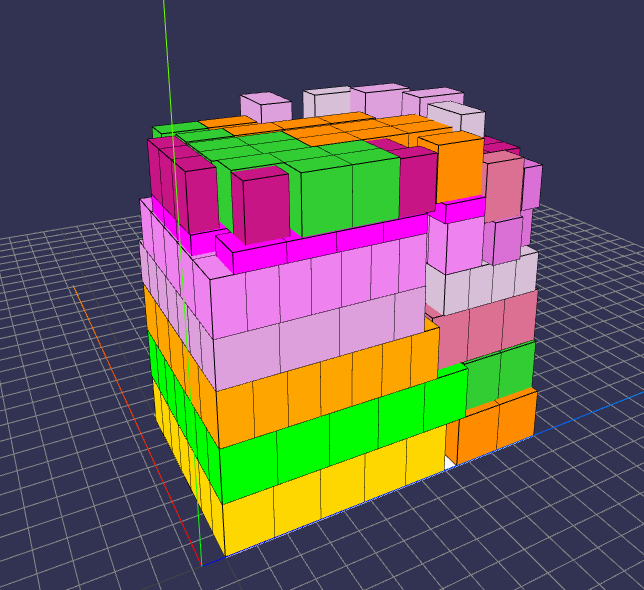
\includegraphics[width = 3in]{tests/usecase/instance-95_k200.PNG}} 
    \subfloat[Instance 82]{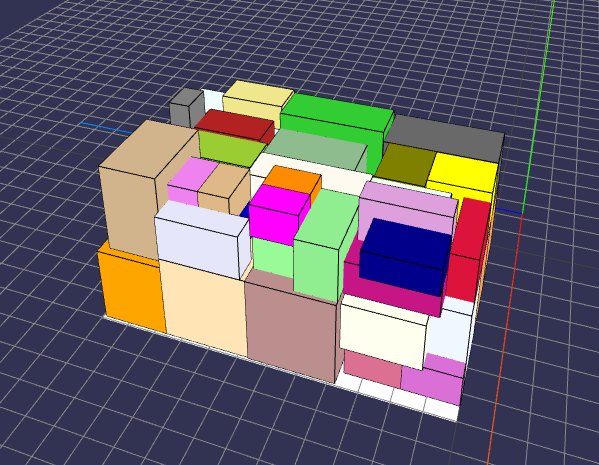
\includegraphics[width = 3in]{tests/usecase/instance-82_k200.PNG}}\\
    \subfloat[Instance 56]{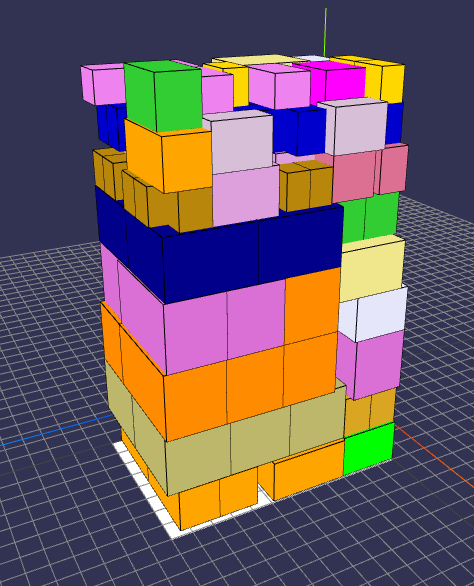
\includegraphics[width = 3in]{tests/usecase/instance-56_k200.PNG}} 
    \subfloat[Instance 66, Bin 1]{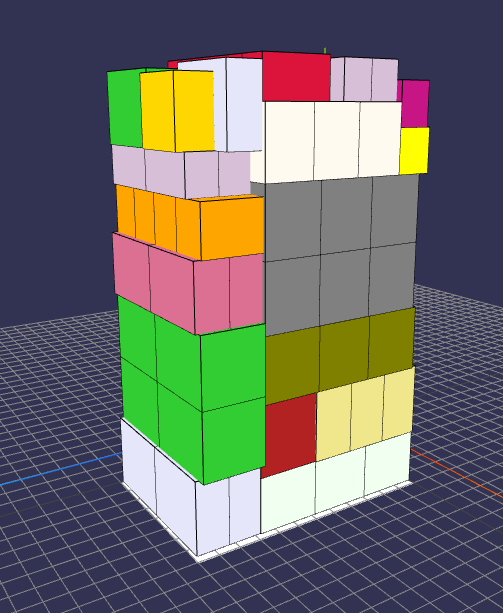
\includegraphics[width = 3in]{tests/usecase/instance-66_bin1_k200.PNG}}
    \caption{Some solutions of the use-case tests with the "Group by Hash" behaviour and $k=200$}
    \label{fig:usecase_tests}
\end{figure}